




%\pagenumbering{gobble}
%\newpage  
%\pagenumbering{arabic}
%\pagenumbering{gobble}

\section{Introduction}
\label{sec:intro}

Fuzzing~\cite{fuzzoverview} is one of the most important recent advances in 
automated software testing.  Modern coverage-driven fuzzers, such as AFL or 
libFuzzer, generally work by maintaing a set (called a corpus) of potentially interesting 
inputs for the program being fuzzed (often referred to as the target).  The corpus may consist of a 
trivial input, or examples of real-world inputs (or test cases), initially.  
The fuzzer then selects one such input, modifies it in some fashion, and 
submits the input to an instrumented version of the program being fuzzed.  If 
the execution produces novel behavior (e.g., covers new code or takes a new 
path through already-covered code), the modified input is added to the set of 
likely-interesting inputs.   If the execution reveals a bug, of course, it is 
saved for inspection.   Fuzzers differ widely in their strategies for selecting 
among interesting inputs, modifying inputs, and determining what constitutes 
potentially interesting behavior worth further exploring, but this broad picture of the basic 
structure of modern, effective fuzzers, is largely applicable, even to fuzzers 
making use of machine learning or symbolic execution techniques.

This basic approach has proved extremely effective in finding bugs, and in the 
shape of OSSFuzz (supported by Google, the Core Infrastructure Initiative and 
the OpenSSF), is used to probe a large number of critical open source systems, 
finding over 8,900 vulnerabilities and 28,000 bugs across 850 projects, to date.

Fuzzing has unsurprisingly become a major topic of academic security and 
testing research, as a result of the obvious power and success of the basic 
technique.  Historically, most such research results in \emph{the development of a 
new fuzzer.}  The most frequently seen kind of research paper in the field of fuzzing
research evaluates a
novel fuzzer developed by the academic researchers against a set of well-known 
fuzzers and recently published academic fuzzers.  Such work often results in 
the availability of new, powerful fuzzers and fuzzing techniques, of course.  

However, in many cases,
the underlying novelty is a relatively isolated concept that ends up being 
embedded in some cases in a more mature but otherwise technically
less-than-sophisticated fuzzer.  For example, 
the first release of the highly successful Eclipser fuzzer~\cite{Eclipser} was very successful, 
due to the power of the lightweight semi-symbolic method used to modify 
inputs in intelligent ways.  However, the research team acknowledged that their 
implementation of more mundane aspects of fuzzing was somewhat \emph{ad hoc}.  The 
second version of Eclipser moved to using the widely used AFL fuzzer~\cite{aflfuzz} to support 
most aspects of fuzzing other than the core innovation.  
%
Moreover, fuzzing advances only appear in new fuzzers 
if later fuzzer developers adopt them as standard practice. When a 
fuzzing advance is not adopted, it can
essentially end up abandoned as part of an outdated fuzzer.   It is
not obvious that researchers \emph{want} to implement new ideas as
(potentially abandoned) forks of existing fuzzers, or as novel,
simple, fuzzers.  Instead, they do not know of any other option,
realistically.  Moreover, researchers are likely aware that fuzzer
evaluation, already a difficult task, is easiest in the context of
comparing a single new fuzzer to a set of existing fuzzers.

There have been some attempts to overcome this problem. For example, 
FuzzFactory~\cite{fuzzfactory} is a generalized fork of AFL which enables researchers 
to instantiate and compose fuzzers with custom feedback functions by only 
instrumenting the target program. Another prominent example is AFL++~\cite{AFLplusplus}, a 
version of AFL incorporating many academic and industrial fuzzing advances, 
into a notably effective fuzzer.  However, there remain many individual 
programs on which some other fuzzer outperforms AFL++. Indeed, the use and
composition of 
many different, even sub-optimal, fuzzers is likely required for truly 
effective fuzzing~\cite{chen2019enfuzz,UsesDiversity,ensemble,pastis}, a key
motivation for the infrastructure this project proposes to build.

\paragraph{Meta-fuzzing.}
These previous efforts generally represent examples of 
\emph{meta-fuzzing}, a promising overall approach to improving fuzzing by 
\emph{moving the fuzzing technique outside the fuzzer itself.}  The simplest 
such approaches to consider are ones based on altering the fuzzing target, 
which is of course common across fuzzers. To illustrate, consider
the problem of decomposing comparisons in a program.  Usually, a fuzzer can only observe if a 
program takes a given branch or not at the binary level.  Decomposition breaks 
down CMP instructions into individual bit-level comparisons (or some other 
appropriate structuring) such that, beyond whether or not a branch was taken,
how \emph{close} the branch is to being taken is also visible to the fuzzer  (analogous to a branch 
distance in search-based testing~\cite{mcminn2004search}).  There exist various alternative versions of 
the basic idea, in e.g., Steelix~\cite{Steelix} and
libFuzzer~\cite{libFuzzer}, which are usually implemented 
as modifications to the fuzzer's custom instrumentation approach.  However, the basic 
idea can also be implemented by transforming the source code of a program to 
expose the structure of a comparison.  The DeepState~\cite{DeepState} property-driven fuzzing 
tool does this for its own assertion implementations, as does FuzzFactory in 
its \texttt{CMP} domain.  Such a transform might take, e.g.:

\begin{code}

if (x == y)
\end{code}

\noindent where {\tt x} and {\tt y} are integer variables, and rewrite the code 
as:

\begin{code}
cmp\_x\_y = TRUE;
bool cmp\_bit\_0 = bit(x, 0) == bit(y, 0);
if (cmp\_bit\_0) \{cmp\_x\_y = FALSE;\}
bool cmp\_bit\_1 = bit(x, 1) == bit(y, 0);
if (cmp\_bit\_1) \{cmp\_x\_y = FALSE;\}
$\ldots$
if (cmp\_x\_y)
\end{code}

\noindent Although inefficient relative to custom binary instrumentation, this
approach has the key advantage it enables \emph{any fuzzer} to make use of the power of 
decomposition, even if the fuzzer developers were unaware that such a technique 
existed. 

While this particular technique, for efficiency reasons, is likely best 
implemented inside a fuzzer's instrumentation pass, other meta-fuzzing 
techniques are truly universal.  For example, in recent work, PIs Groce and Le Goues 
proposed fuzzing based on program mutants~\cite{fuzzing22}, which modifies a fuzzing 
target in a large variety of ways.  Results show that this approach, by 
allowing a fuzzer to explore program branches in non-chronological order, can 
improve the performance of even state-of-the-art fuzzers such as AFL++, 
as benchmarked by Google's FuzzBench.  The particular approach taken
by this work was inspired by T-Fuzz~\cite{tfuzz}, which in some sense
clearly was \emph{conceived} as a meta-fuzzing approach, but implemented as a
fairly complex standalone
tool that as a result of this choice is no longer maintained or usable.  A key
goal of this project is to avoid \emph{lost work} such as is
represented by T-Fuzz, by providing tooling offering fuzzer developers
tools for implementation and evaluation that are more powerful and
even more convenient than the unfortunate baseline of ``forking and hacking AFL and benchmarking
the resulting tool.''

A core tenet of meta-fuzzing is that the fuzzing tool need not be aware of what 
the program transformation is trying to achieve. For example, in the 
FuzzFactory framework~\cite{fuzzfactory}, co-PI Padhye demonstrated that new 
fuzzing applications---such as finding worst-case performance or 
memory-allocation bottlenecks, as well as targeting fuzzing towards specific 
program locations---can be instantiated by only transforming the target program 
and using an API to send domain-specific feedback from program execution in the 
form of key-value maps. Padhye also demonstrated that composing program 
transformations, achieved by combining key-value maps across multiple 
FuzzFactory domains (such as breaking down CMP operations and tracking 
\texttt{malloc}'d memory), can produce results that are better than applying 
each transformation individually.

\paragraph{Ensemble Fuzzing.}   Ensemble fuzzing \cite{chen2019enfuzz,ensemble,pastis} is an 
approach that recognizes the need for
diverse methods for test generation, at least in the context of
fuzzing.   Inspired by ensemble methods in machine learning 
\cite{dietterich2002ensemble},
ensemble fuzzing runs multiple fuzzers, and uses inputs generated by
each fuzzer to ``feed'' other fuzzers, since different fuzzers have widely 
differing strengths and weaknesses. Ensemble fuzzing is, by nature, a 
meta-fuzzing approach, in that it uses individual fuzzers as ``black boxes'' 
that take in inputs and a program and produce novel inputs of interest.  
Ensemble fuzzing is an extremely promising approach, given that in most 
large-scale benchmarks of fuzzers, there are times when the best fuzzers 
overall perform poorly for some targets, and when the worst fuzzers perform 
well.  The future of fuzzing likely lies in ensemble methods, but the 
implementations proposed thus far tend to 1) not be supported long, and soon 
fail to work at all 2) and/or are limited to very simple naive strategies for 
allocating resources and sharing seeds. This
project aims to make it easy to 
experiment with \emph{sophisticated} ensemble fuzzing approaches, without 
worrying about the infrastructure of executing fuzzers or extracting feedback 
to use in resource allocation.

\paragraph{Target Transformations.}  While ensemble fuzzing is ``meta'' in that 
it uses multiple fuzzers largely as black boxes, another approach largely 
dispenses with direct interaction with fuzzers at all.  As the example above 
suggests, one fuzzer-agnostic way to change the behavior of a fuzzer is to 
change the fuzzing target itself.  This is most easily done at the source 
level, in essence producing a (slightly) different program to fuzz.  In some 
cases, though, binary transformation may be required because the
source for a program is simply not available.   Transformations may be used to make aspects of 
program behavior more visible as coverage, as in the simple example, or to 
improve the oracle for fuzzing, transforming more behaviors into fuzzer-visible 
crashes.  More ambitiously, as in the prior work of PIs Groce and Le Goues, a 
transform may change the behavior of fuzzing algorithms.  Fuzzing program 
mutants allows fuzzers to detect ways to cover branches that, without 
transformation, would not have been executed yet, improving fuzzer 
effectiveness dramatically in some cases.

\paragraph{Universalized Custom Mutators.}  One feature supported by
the widely used fuzzers AFL++ and libFuzzer as well as the promising
new fuzzer Centipede (which backs Google's FuzzTest
project~\cite{fuzztest}) is the introduction of custom mutators:  user-written 
additional ways to modify inputs to generate new inputs.  While changing the 
mutation strategy of a particular fuzzer can be a highly fuzzer-specific 
method, focusing on some unusual coverage or ``magic byte identification'' 
element of the particular fuzzer, many custom mutators are naturally fuzzer 
agnostic.  For example, PIs Groce and Le Goues introduced custom mutators for 
fuzzing compilers that resulted in the detection of hundreds of subtle compiler 
bugs \cite{cc2022}. These were unfortunately implemented in a standalone variant of the 
original AFL fuzzer, but would be more widely used and more effective if 
implemented as custom mutators for libFuzzer, AFL++, and Centipede.  We propose to support 
research along these lines by allowing users to write a single custom mutator 
in a generic byte-based framework, and provide wrappers to integrate such 
mutators into all fuzzers that support custom mutators.

\paragraph{Domain-Specific Meta-Fuzzing.} The above summaries introduce 
broad classes of meta-fuzzing approaches, and we briefly introduced  
general-purpose meta-fuzzing techniques (e.g., the use of program mutants to 
explore branches non-chronologically).  Meta-fuzzing can also be used for more 
domain-specific purposes, however.  Consider the problem of testing machine 
learning (ML) algorithms in general, and specifically neural network 
implementations.  Using off-the-shelf fuzzers directly on ML systems is usually 
ineffective, because the behavior of the system is not primarily encoded in the 
source code of the system, and thus visible to code coverage instrumentation.  
Instead, \emph{data} in the form of a neural network, decision tree, etc. 
determines the system behavior.  The ``code'' to be explored is not visible to 
traditional compiler instrumentation.  A meta-fuzzing approach to this problem 
would be to define transformers that understand the nature of a machine 
learning implementation (the standard libraries used widely to implement ML 
systems) and use the data encodings to produce \emph{source mirrors} that take 
inputs to the ML algorithm and produce visible code coverage for a fuzzer.  One 
aspect of our general meta-fuzzing infrastructure, discussed in more detail 
below, is to additionally to support domain-specific fuzzing that falls outside 
the locus of ``fuzzing Linux application binaries'' previously centered in 
fuzzing benchmarking.


\paragraph{The Problem of Evaluation.} Evaluating fuzzers is, even in the 
current common setting, where evaluation is usually of a single ``new'' fuzzer, 
a complex problem. Many evaluations in the literature are insufficient or even 
incorrect~\cite{FuzzerHicks}.  Evaluating meta-fuzzing adds a further quantitative (and to some 
extent qualitative) element to this problem: rather than comparing a single 
fuzzer to a set of competing fuzzers across benchmarks, evaluating meta-fuzzing 
methods involves evaluating a \emph{set} of fuzzers $F_1 \ldots F_n$ against 
$F'_1 \ldots F'_n$ (where some meta-fuzzing method has been applied), and 
determining the degree of improvement or degradation in effectiveness in each 
case.  This alone would make support for benchmarking and comparing fuzzers an 
important feature of any framework for meta-fuzzing research and development.  
However, as noted above, future ensemble methods are likely to also make use of 
fuzzer evaluations to allocate resources.  Therefore a major thrust of this 
effort is to adapt the aspects of the framework that support ensemble fuzzing 
to support measurements of fuzzer effectiveness as well.  This feature of 
course has applications beyond meta-fuzzing methods; traditional fuzzer 
evaluations can also be expected to benefit from a systematic, 
multi-measurement framework for running a set of fuzzers on multiple
benchmarks.  However, our central motivation is that we expect that the complexities of running
meta-fuzzer evaluations have tended to discourage implementation of
clearly-meta-fuzzing ideas in any form but that of a single new fuzzer
or fuzzer fork.


%\adg{Do we like this?   Jason can you draw a diagram if we do?}
\begin{figure}
\centering
% fbox to help visualizing trimming
%\fbox{
% Answer: [trim={left bottom right top},clip]
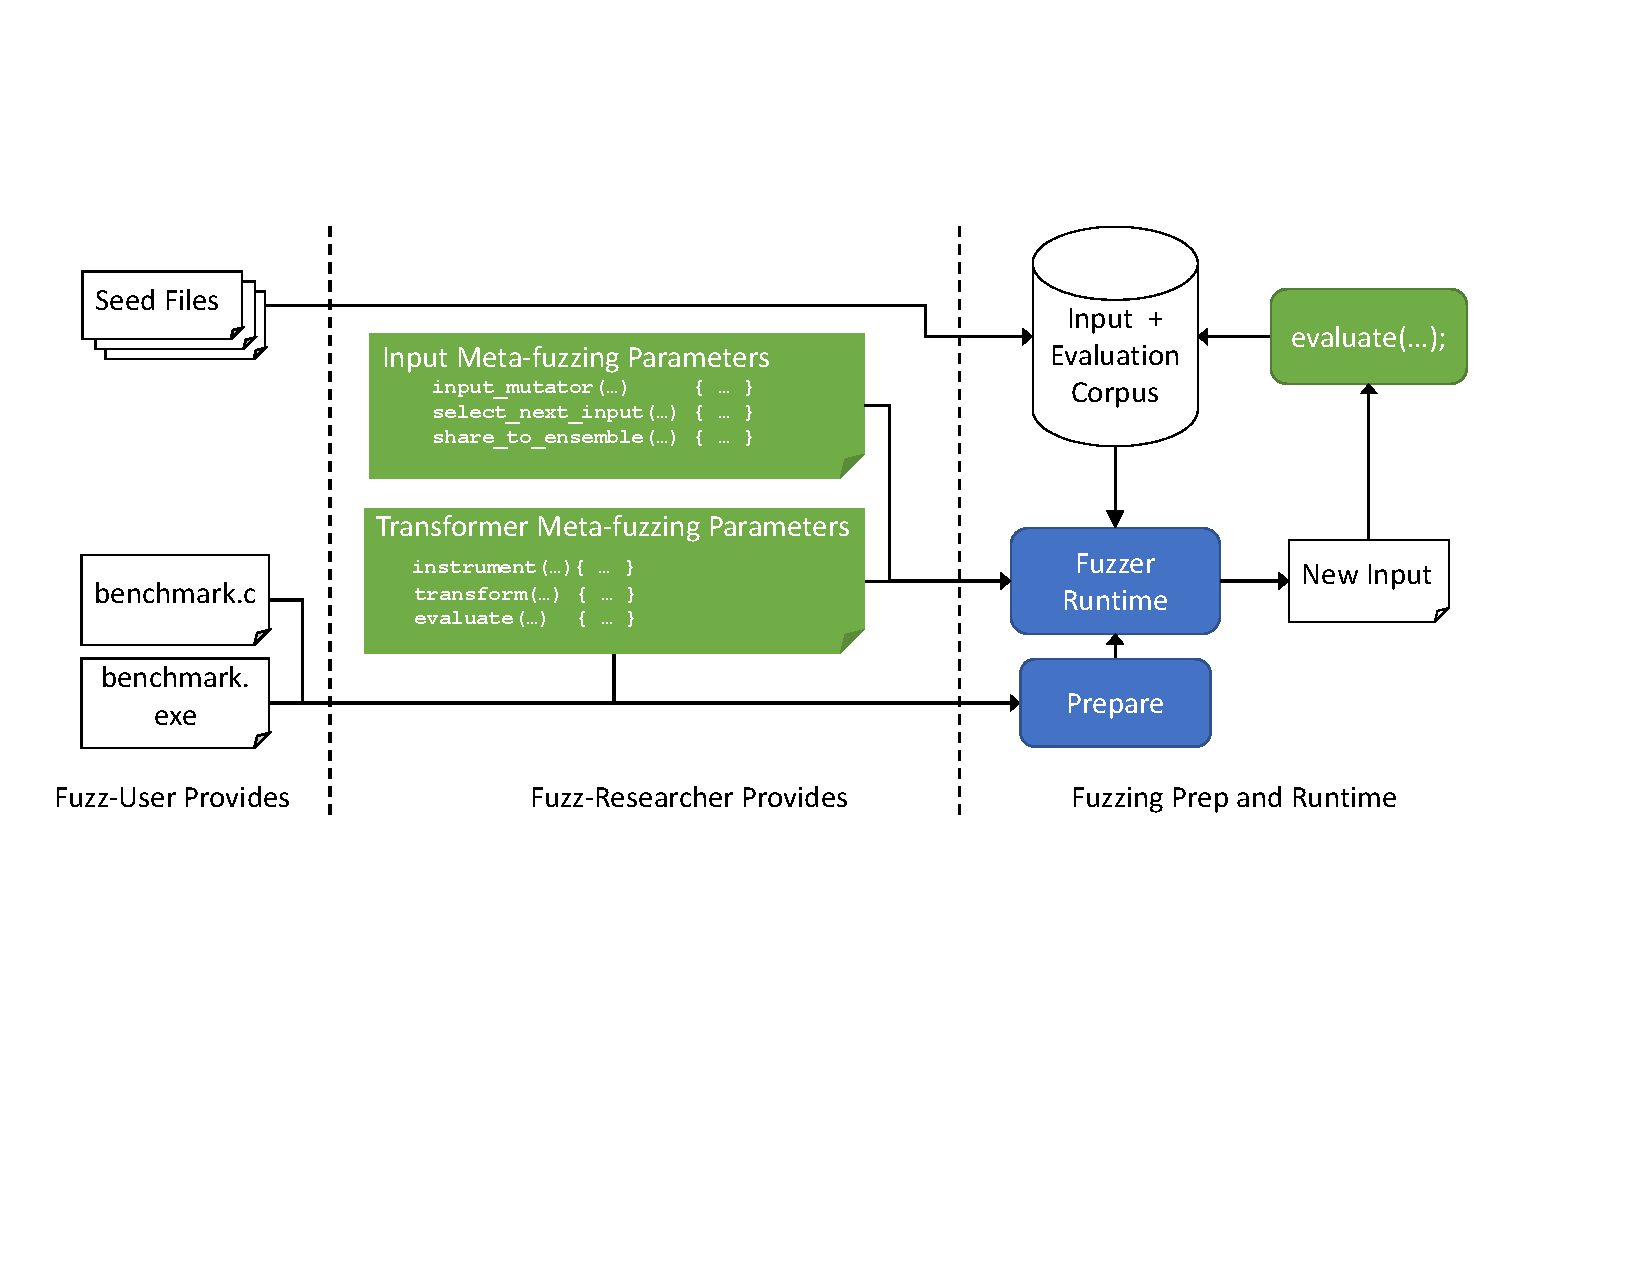
\includegraphics[width=0.8\textwidth,trim={0.3in 3.0in 1.2in 1.4in},clip]{figures/fuzzer-arch.pdf}
%}
\caption{A view of a generic meta-fuzzer.}
\label{fig:meta}
\end{figure}

\paragraph{The Big Picture.}  Meta-fuzzing is perhaps best understood
as follows: a modern fuzzer is a tool that, fundamentally, takes in
two kinds of input, and produces tests (new inputs) as outputs.  The
two kinds of inputs are:  the corpus inputs/tests, and (less
obviously) the target program to be fuzzed.
Traditional fuzzing research changes the ``fuzzing function''
itself, and thus must be implemented for every fuzzer to be
used. Meta-fuzzing, by contrast, changes the \emph{inputs}, and so can
be agnostic as to the underlying fuzzer.   Ensemble fuzzing works by
changing the corpus inputs, drawing them from the outputs of another
fuzzer.  Universal custom mutators change the set of
inputs executed by the fuzzer, by adding transformations to the
repertoire of multiple fuzzers.  Source and binary transformations
modify the program to be fuzzer, either once (often to add coverage
visibility or further ability to detect crashes) or by producing many
verisons of a program, in order to allow fuzzers to better explore
behaviors of the program.  Figure~\ref{fig:meta} shows meta-fuzzing as
a set of functions operating on fuzzer inputs.  The underlying concept
of this proposal is that researchers need tool support to enable them
effectively develop and evaluate functions for meta-fuzzing.




\subsection{Overview of Proposed Work}

This project proposes, first, to create a reliable infrastructure for executing 
multiple fuzzers on a set of targets and collecting data from these executions. 
 Such data includes generated inputs and detected bugs, of course, but also 
measurements of fuzzer effectiveness, e.g., code coverage of corpuses and 
incremental code coverage.  This infrastructure will be able to run locally for 
debugging and quick turnaround, and will support cloud deployment for 
large-scale experiments. Critically, this infrastructure will be designed to 
support ensemble fuzzing and complex ensembling strategies, from the ground up; 
support for exchange of generated inputs and shifts in resource allocation will 
be built-in, rather than added on, and a high-level declarative language for 
describing ensemble strategies will allow researchers to explore the space of 
ensemble methods.

A second key element of the proposed system is the development of tooling for 
expressing source and binary-level transformations to support meta-fuzzing 
methods that rely on modifying the target to be fuzzed.  Such methods may focus 
on making more behavior of a system visible to fuzzers within the paradigm of 
``source coverage'' currently supported by essentially all modern fuzzers, or 
on enhancing oracles to enable all fuzzers to detect larger classes of bugs, or 
on transformations that target the underlying logic and bottlenecks of fuzzing, 
such as the non-chronological exploration of branches enabled by using program 
mutants.  This thrust, again, will focus on providing a way for researchers and 
developers to easily express such transforms and deploy them across a large set 
of fuzzers.

Third, the proposed system will included facilities to allow researchers and developers to 
write custom mutators for fuzzers in a fuzzer-independent way, with support for 
automatically generating wrappers to run these ``universalized'' mutators 
inside the fuzzers (including AFL++ and libFuzzer) that 
support custom mutators.

Finally, the proposed system will allow meta-fuzzing of domain-specific applications
which traditionally have been incompatible with conventional fuzzing tools and
benchmarking platforms that expect targets to be single-process programs with
a well-defined input and execution interface.

\subsection{Qualifications of the Project Team}

{\bf Lead PI Alex Groce} is a well-known expert in fuzzing and software testing
in general. While he has been in academia since 2009, his research is informed
by experience as the lead for testing fight software systems at NASA/JPL,
including a lead role in testing the file systems for the Curiosity Rover. He
has also continued to work on practical tools, as lead developer for four open
source tools hosted on GitHub with over 100 stars (one with over 700
stars). His expertise in fuzzing and
practical testing is widely known, and in 2021 he was hired to perform an audit
and contribute enhancements to the fuzz testing for the primary reference
implementation for the Bitcoin blockchain, a critical system with more than 71
thousand GitHub stars, on which the validity of billions of dollars worth of
financial transactions relies.

Co-PI Padhye has substantial expertise in grey-box fuzz testing~\cite{perffuzz,
jqf, zest, fuzzfactory, rlcheck, bigfuzz, bonsai, naturalfuzz, mu2}. In
particular, his past work on controlling fuzzers' input search space~\cite{jqf,
zest}, on customizing the feedback function in grey-box fuzzing
algorithms~\cite{perffuzz, fuzzfactory, bonsai, mu2}, and on targeting
domain-specific applications~\cite{partemu, bigfuzz, naturalfuzz} is
particularly relevant to this project. Padhye has a track record in developing
and maintaining open-source software such as JQF+Zest~\cite{jqf-github} (577
GitHub stars) and FuzzFactory~\cite{fuzzfactory} (225 GitHub stars).

Co-PI Le Goues has expertise in novel techniques for automated
source-level program transformation, and its application.  A key example is the
Comby language/tool for automatically searching over and transforming code in a
language-agnostic way~\cite{rvt-ppc,comby-github}.  Her work has applied transformation in a number of
contexts, including but not limited to fuzz testing~\cite{cc2022}, 
program repair~\cite{wong21varfix,legouesNFWTSE2012,footpatch}, API migration~\cite{ni21soar}, fuzz test
triage~\cite{vantonder-ase18}, and static analysis customization~\cite{vanTonder-tailoring20}.  She
also has a track record for releasing and supporting open source research
artifacts, including the Comby language (more than 2200 GitHub stars) and the
widely-used ManyBugs benchmark~\cite{legoues15tse} for evaluating automatic program
repair techniques.

Co-PI Davidson, and key Senior Personnel Hiser and Nguyen-Tuong have significant
experience with binary program transformations, and both source-based~\cite{ahmed2021bigmap} and binary-only fuzzing~\cite{nagy2021breaking,nagy2021same}.
Their open-source Zipr binary rewriting infrastructure has been used in several
projects to retrofit binaries with security hardening transformations~\cite{zipr,hawkins2017zipr,hawkins2017securing,hiser2017zipr++,schulte2022broad}, including
the DARPA Cyber Grand Challenge~\cite{nguyen2018xandra}, and more recently, an NSF project to automatically harden and diversify VM images
to protect open-science infrastructures~\cite{davidson2023helix++}. 
Zipr provides the technological foundation for ZAFL, their highly-efficient AFL-compatible open source binary fuzzer~\cite{zafl}.
Key to ZAFL's efficacy is the integration and stacking of modular fuzzing-enhancing program transformations~\cite{nagy2021breaking,nagy2021same}.

\subsection{Intellectual Merit and Broader Impacts}

\paragraph{Intellectual merit.} The proposed work will advance the
knowledge and understanding of software testing by enabling
researchers and developers to conduct scalable experiments in meta-fuzzing.  
Meta-fuzzing approaches rely on the development of theories and heuristics 
about the exploration of program behavior, or the optimal allocation of 
resources to fuzzing tools, that apply without reference to specific underlying 
fuzzing algorithms.  Such approaches therefore, in addition to providing 
practical tools for finding bugs in code, advance our knowledge of the behavior 
of software systems.

\paragraph{Broader impacts.} Advancing the effectiveness of fuzzing can improve 
software testing in general and
thus software quality, benefiting (directly or indirectly) all
segments of society that depend on software.  The grant
will also support several graduate and undergraduate students, giving them 
experience with
building software artifacts and performing empirical studies.


\section{Key Deficiencies of Existing Infrastructure}

To our knowledge, \emph{no} infrastructure exists for performing 
\emph{fuzzing-specific} source or binary transformations of programs, or writing 
custom mutators that can be used by more than one fuzzer.  While
fuzzers can share corpuses, and there are commonalities to
instrumentation formats across the AFL family, there is to our
knowledge no tool support for exploiting these commonalities (e.g.,
adding new instrumentations based on novel source patterns).  These aspects of meta-fuzzing fit into the picture of a promising 
research area with, essentially, no available tooling beyond individual 
fuzzers, outside the area of ensemble fuzzing.

In ensemble fuzzing, in addition to some deprecated projects, or ones of 
limited applicability, there is the PASTIS framework~\cite{pastis}.  PASTIS was used to place first, tied 
with {\tt afltrusttrust} in the bug-detection category of the 2023 SBFT fuzzing 
competition~\cite{toolcomp}.  However, PASTIS at present only supports
AFL++, Honggfuzz, 
and the symbolic execution tool TritonDSE.  Infrastructure to add more fuzzers, 
however, is present.  More importantly, PASTIS uses an extremely simple 
strategy:  it shares all seeds detected with all fuzzers and symbolic execution 
engines, and does no allocation of different resources to different fuzzers.  
Given the critical problem of fuzzer saturation, in settings with limited CPU 
resources (essentially all settings, given the number of available viable 
fuzzers and resource hunger of fuzzers), in the long run applying more 
sophisticated methods, e.g., from multi-armed bandit optimization (and in 
particular ``rotting bandit'' \cite{levine2017rotting}) settings is critical for effective 
ensemble fuzzing.

Because PASTIS performs no resource allocation, it also relies on other 
infrastructure to perform any evaluation of the fuzzers being used in the 
ensemble, or of the whole strategy.  The SBFT contest and some recent research 
has used FuzzBench, a service provided by Google~\cite{metzman2021fuzzbench}.  However, FuzzBench is 
somewhat notoriously difficult to use and often produces failures, even for 
``core'' fuzzers such as AFL++, on some benchmarks, that prove difficult 
to diagnose or debug.  It is at best highly unclear how much support Google 
plans to devote to FuzzBench in the future.  FuzzBench is also deeply
tied to Google cloud infrastructure, which means that practical use of
the system is not feasible if Kubernetes, openstack, AWS, or another
cloud approach is better for a particular user.

The connection between fuzzer 
benchmarking and evaluation and ensemble fuzzing is, we note, clear enough that 
an (abandoned) attempt was made to transform FuzzBench 
into a rudimentary ensemble fuzzing tool~\cite{fuzzbenchensemble}.   Other fuzzing benchmarks, such as 
MAGMA~\cite{MAGMA}, are often tied to a specific set of benchmarks, with manual effort to 
make them fit into the framework, and so are not obviously suitable as a basis 
for ensemble fuzzing (and general evaluation purposes).  PASTIS, FuzzBench, and 
MAGMA all may provide useful insights into possible approaches to the core 
infrastructure of our ensemble fuzzing/fuzzer evaluation component, but none 
are, themselves, currently suitable for the purpose, and the benchmarking 
systems are even limited in usability for that purpose.   Their
inherent focus on comparing fuzzers given fixed resources is not
general-purpose enough to be suitable for allocating limited resources
on the fly, as they stand.


Source and binary transformation systems do exist, of course, but none are 
aimed at meta-fuzzing, which likely would strongly benefit from a 
Domain-Specific Language focused on making it easy to express the kinds of 
tranforms (in particular, introduction of ``mirror'' coverage structures to aid 
visibility) useful in meta-fuzzing.  Moreover, for binary instrumentation, some 
awareness of the instrumentation produced by various fuzzers is critical if 
transforms are to avoid modifying code that the fuzzer relies on working in a 
certain way.  In the extreme case, rather than simply producing incorrect 
instrumentation (e.g., coverage) results, such modifications could make a 
target completely unusable, by always triggering a crash of the target.

\section{Infrastructure Description}

\subsection{Fundamental infrastructure}

\subsection{Thrust 1: A Foundation for Efficient Fuzzer Execution,
Orchestration, and Evaluation}

An infrastructure for (meta-)fuzzing research, 
whether for evaluating large sets of fuzzers in a (meta-)fuzzing approaches, 
evaluating architecture-specific fuzzing feature benefits, 
or for less-explored but promising research such as determining which kinds of 
fuzzers work best for broad classes of fuzzing, needs to be sufficiently 
efficient, robust and configurable to support a variety of (possibly 
unforeseen) requirements.  
Further, this infrastructure needs to be easily extendable to support new input 
mutators, benchmarks, input sharing, and new computation-providing backends 
(e.g., a new version of OpenStack.)

We propose an infrastructure, as shown in Figure~\ref{fig:overview} that meets these many various needs by focusing on 
simplicity and extensibility.  We propose a simple API based on separating the 
provisioning of hardware resources that installs an execution agent on the 
provisioned hardware.   The execution agent, running with elevated privileges, 
talks to a centralized server to coordinate a fuzzing.  It reports back 
available hardware resources.  The central server instructs execution agents on 
packages to install, fuzzing campaigns to start, fuzzing parameters such as 
which mutator to use,, during- and post-campaign statics to request, etc.  The 
fuzzing-campaign director interacts with the server to configure, start, 
monitor, interrupt, or gather statistics from a fuzzing campaign.  Further, a 
campaign director can upload a previously created configuration to the server 
to launch a campaign, allowing for repeatable operation..  

The infrastructure will come with pre-configured fuzzing campaigns, fuzzer 
configurations, input sharing schemas, and VM images to allow easy adoption for 
beginning users.  We plan to initially target OpenStack leveraging the UVA 
hardware resources available, as well as CloudBank AWS/Azure.

Lastly, the configuration options will focus on general meta-fuzzing strategies 
to allow for easy user extensibility.  End-users will be able to easily create 
new fuzzing components (e.g., input mutator, code instrumentation type, input 
sharing mechanisms) by writing new configuration files, schemas or 
pre-configured machine images.  The collaborative effort will attempt to accept 
community-submitted extensions to our proposed open-source infrastructure when 
the project has achieved a minimal level of acceptance.

The following thrusts describe in more detail how meta-fuzzing can be realized 
in the proposed infrastructure.


\begin{figure}[htbp!]
%\makebox[7in][7in]{to be filled in}
\vbox to 7in {\vfil
\hbox to 7in{a figure to be drawn later}%
\vfil
}

\caption{Proposed Meta-fuzzing infrastucture overview.  
A fuzz-campaign director interacts with the meta-fuzzer server to setup or replay a configured fuzzing campaign.  
Built-in collections of of benchmarks, machine images, input sharing techniques, hardware resource requirements, input mutators, and other fuzzer configuration 
allow for quick startup of fuzzing campaigns backended by popular cloud service providers as well as configurability and extensibility for custom fuzzing setups.  
The system allows an experimentor to quickly and simply obtain results, or reproduce prior fuzzing campaigns.}
\label{fig:overview}
\end{figure}



\cut{

	\subsection{Thrust 1: A Foundation for Efficient Fuzzer Execution,
Orchestration, and Evaluation}

The execution of large sets of fuzzers for purposes of evaluating
(meta-)fuzzing approaches, or for less-explored but promising research such as
determining which kinds of fuzzers work best for broad classes of fuzzing
targets (e.g., compilers, media parsers, data structures, etc.) is essentially
the same core task as that required for sophisticated ensemble fuzzing.  The
only real difference is that a benchmarking run 1) runs all the fuzzers with
the same resource allocation and 2) there is no sharing of inputs between
fuzzers.  That is, fuzzer benchmarking is a simplified, restricted, version of
what is needed for a successful platform for implementing ensemble fuzzing.
The core needs are the same: ease of adding new fuzzers and including new
targets, ease of deployment to both local environments (for easy debugging or
use in developer ``unit fuzzing'') and the cloud (for large-scale fuzzing or
fuzzer evaluation), and ability to produce easily interpretable, statistically
usable, results (for both human consumption and resource allocation).

\jdh{UVA can you talk more about how to go about this thrust?}

fuzzers -- which fuzers to use, and how to extend infrastructure for new 
fuzzers.  This is really NAU?
benchmarks -- standard fuzzing benchmarks, plus ability to add custom 
benchmarks.
specification -- which backend to use, how to allocate resources, how a fuzzing 
campaign should look like, which mutators to use, which instrumentation to use.
deployment -- VM allocation, software installation, efficient (semi-)automatic 
assignment of fuzzers based on fuzz campaign mapping
cooperation -- how often to share, and what to share.  Sharing "architectures" 
(e.g., share on the same VM, vs. different VMs in same cluster vs VMs in 
different clusters vs VMs in different data centers)
results -- collecting results (baseline results + user-specified extensions), 
statistical analysis


}



\subsubsection{Expressive Source and Binary-Level Transformations to 
Enable Meta-Fuzzing}

The key problem in enabling target transformation to enable meta-fuzzing is to
provide a flexible, expressive mechanism for describing a wide range of useful
transformations, at both the source and binary level.  It is important that this
mechanism be natural and accessible to users; forcing users to 
construct complex ways to express each transform will frustrate exploration of such 
techniques and result in buggy implementations. 

For source-level transformations, we will incorporate (and lightly extend) the
Comby tool and language~\cite{rvt-ppc,comby-github} into the metafuzzing
framework.  Comby is a tool and language for declarative syntactic program
transformation that applies to multiple languages. Comby is both more usable and
more powerful in terms of the types of transformations that it can express than
regular expressions, while being more efficient and general than heavyweight
language-specific approaches. The key innovation is to convert declarative
transformation templates into parsers that directly match and transform source
code of interest. Parser combinators~\cite{Hutton96monadicparser} define how to
match nested structures (much like traditional AST visitor traversals) but
without the need to define or build an intermediate AST. This is highly
performant and largely language agnostic, and allows users to express desired
transformations in natural syntax that is very close to the underlying source
language. 

To ease the use of Comby in this context, we will implement a set of wrapper
macros for Comby customized to the particular task of converting desired
properties into static, coverage-visible code constructs.  We will additionally
produce a library of existing transformations that are useful or common in prior
meta-fuzzing approaches, both to amortize uptake and demonstrate the use of the
approach.  

As part of this effort, we will identify important transforms common to current
and upcoming meta-fuzzing algorithms.  We will use these existing desired
transforms to inform our design of the Comby templates that enable their
application. These templates will effectively serve as a DSL that enables users
to concisely describe desired predicates over some dynamic data value or
behavior, to be translated into a static coverage construct in code. 

%\clg{Question: OK, in the above I basically said we'll make a bunch of Comby macros that can
%express many different types of transformations, including extant
%transformations and potentially new ones.  I thought this seemed less
%complicated than saying we'll make a NEW DSL.  But, if we want to express all
%transforms, binary or source, in a COMMON DSL, that's a slightly different
%story.  So, question for UVA: how best to configure or express a system of
%binary-level transformations for this purpose?}



For binary-only program instrumentation, Comby is unsuitable as it requires source to operate.
Instead, we leverage the robust binary rewriting techniques provided by Zipr.~\cite{hawkins2017zipr, hiser2017zipr++,zipr}
Zipr has undergone rigorous third-party evaluation involving thousands of binaries spanning across about 50 unique programs
compiled with various compilers and compiler flags and seen no failures.~\cite{schulte2022broad}
Zipr's plug-in architecture allows arbitrary insert, delete, or modification of 
code or data items as well as allowing plugins to be composed, making it ideal for meta-fuzzing.  
In fact, PI Davidson and the UVA senior personnel,
Dr. Hiser and Dr. Nguyen-Tuong, have already leveraged it to build an 
AFL-compatible instrumentation plugin for Zipr, called
Zafl.~\cite{zafl}  
Experiments show that Zafl instrumentation provides the same
coverage and bug-finding effectiveness as compiler-inserted instrumentation.~\cite{nagy2021breaking}
Zafl also supports input-program mutation to enable faster fuzzing with techniques such as Intel LAF 
(which converts word-length \textit{cmp} instructions to byte-compare instructions similar to what was 
shown in Section~\ref{sec:intro}) or adding temporary breakpoint instructions to
run most coverage tracing at zero overhead.~\cite{intel2016circumventing,nagy2021same}
Zafl has the program mutation and instrumentation passes in separate Zipr plugins, allowing a user to mix-and-match
transforms (in a very meta-fuzzing manner) to suit the needs of their program.

As part of this effort, we will integrate Zipr and Zafl and allow people to extend the binary-only fuzzing
capabilities by adding new plugins to the infrastructure.  We do not expect significant effort to be used to 
develop these already robust components, allowing the infrastructure to leverage their capabilities in to help
build future binary-only meta-fuzzing transformations.


This work will be divided into two sub-thrusts, one for source-level and one 
for binary-level transformations, with PI Groce coordinating work to determine 
if common DSL elements exist, i.e., transforms that can be applied at either 
level.


\subsubsection{Universalized Custom Mutators}

This thrust is concerned with making it possible to write custom mutators for 
multiple fuzzers in a single format, with a wrapper (or source transform) 
specializing this to individual fuzzers.  This is not as simple as it
seems; the interface for custom mutators in libFuzzer and Centipede is
relatively simple, a transformation of a byte buffer; in contrast,
AFL++ supports a complex API using standalone libraries for custom
mutators, requiring substantial effort on the part of implementors at
the gain of additional functionality.  A workable solution for fuzzing
advances that can be represented as mutators (which might even extend
to methods such as Eclipser's approximation of symbolic execution)
needs to accomodate developers who only need a ``libFuzzer'' style
mutator, and automatically supply AFL++ with derived versions for
other calls, as well as those wishing to define the full AFL++ API but
derive a libFuzzer mutator. For the former, automatically applying
AFL++ {\tt afl\_realloc} calls when needed is also critical.

As a first task in this thrust, we propose to re-implement the compiler-fuzzing 
tool developed by PIs Groce and Le Goues as a custom mutator.  By focusing on a 
practical task, we will be able to best perceive difficulties and needs of 
custom mutator implementors, and can produce a library of useful byte and 
code-level mutators to be applied by users.

\subsubsection{Domain-Specific Fuzzers (Cross-Cutting)}

Fuzz testing is useful in many domains where the target is not necessarily a single program that
provides a well-defined input interface, as expected by conventional fuzzing tools such as
AFLplusplus and libFuzzer. For example: web browsers, mobile applications, and spreadsheets 
are reactive systems, always listening for user events. Further, conventional fuzzing tools 
expect that programs terminate quickly after execution, and are easily reset 
for the next trial in a fuzzing loop. However, in stateful domains like database systems 
or networking controllers, a sequence of inputs may drive the target into different states
depending on the order in which inputs are received. Effective fuzzing in such domains requires
carefully defining what a single fuzzing trial looks like. Finally, whether source or binary 
transforms are available, the behavior of programs in some domains may not be related to
any sense of ``code coverage''. For example, in machine learning and data analytics domains,
we may be more interested in the data-flow (e.g., neuron activations or 
data-parallel join operations, respectively) rather than the control-flow in terms of 
conditional jumps. For all these reasons, domain-specific fuzzing has so far been a niche where
researchers are unable to use a common platform for exchanging results and re-using components
such as algorithms, heuristics, and mutators.

In this thrust, we propose to extend meta-fuzzing support to domain-specific applications by
providing a set of interfaces that allow domain-specific targets to be configured on our
infrastructure. The interfaces will allow researchers to define the notion of an ``input'',
a ``trial'' (i.e., a single execution on a given input), and various domain-specific vocabulary
for collecting feedback and evaluating the strength of candidate fuzzers (e.g., replacing ``code
coverage'' with something else). 

This thrust is cross-cutting because it enables the use of our proposed source and binary 
transforms as well as custom mutators in addition to our fundamental meta-fuzzing execution
infrastructure on a variety of application domains which so far have been 
sidelined in the research community.

\subsection{Tools, resources, and datasets}
The full meta-fuzzing software stack presented in the preceding section will be delivered via GitHub or open source repositories as code, data and documentation artifacts. By design, our framework is designed to be extensible for all common facets of the fuzzing operational lifecycle. Thus, incorporating enhancements (e.g., new fuzzers, new transformations, new forms of feedback, new benchmarks, new ensemble methods, etc.) will be a continual and ongoing process, initially performed by our team, but if truly successful, by the community at large. 

%\subsubsection{Benchmarks}

\subsection{User services}
\label{sec:user-services}
%\clg{from the call: ``describe services to be integrated into the infrastructure, including 
%mechanisms by which researchers will gain access to the infrastructure;''}
%\clg{I'm wondering if one of the subsections I initially grouped under 
%tools/resources/datasets might fit better down here.}

% User Services

A good first impression will be key in engendering trust in our meta-fuzzing infrastructure.
Thus, we will provide ready-made images (Docker or VM) so that users can experience
the end-to-end system depicted in Figure~\ref{fig:overview}.
We will provide a suite of such images, pre-configured with various combination of
fuzzers (e.g., AFL++, LibAFL, libFuzzer), 
fuzzing styles (e.g., whole program, library-based, source, binary), 
and benchmarks (e.g, OSS Fuzz benchmarks, programs written in
different languages).

A key element of the infrastructure is that adding fuzzers and
benchmarks must be servicable. For example, users should be able define the
``ports'' the fuzzer accesses, in the vision of Figure~\ref{fig:meta},
e.g., where a fuzzer looks for new seeds when running in ensemble
mode, whether it takes an uninstrumented binary or requires binaries
to compiled, and so forth.  Given a simple DSL for this kind of
extension, adding a new fuzzer should potentialy require almost no
effort in many cases.  However, for fuzzers with complex build or
runtime workflows, e.g., ones requiring multiple binaries such as
Angora, users will be able to provide full scripts defining fuzzers,
as in FuzzBench.

We will actively develop and maintain user documentation, cookbooks and tutorials throughout
the duration of the project. We will support both users that want to just use the system
as well as those researchers that wish to extend the system.
In general, our tutorials and documentation of meta-fuzzing workflows will be
represented and concretized in ready-made images.

One service to the community our approach will offer is to reduce the
risk of performing improper evaluations of fuzzing research.  We aim
to clearly indicate community-expected standards for fuzzer
evaluations~\cite{FuzzerHicks}, document aspects of configuration that
are concerned, and set the defaults for our infrastructure to perform,
when not modified, high quality fuzzer evaluations.

We will host our software repository on GitHub and use standard GitHub facilities
to manage interactions with end users, e.g., issues, pull requests, discussions, feature requests.
Over time, other researchers and practitioners will extend the base infrastructure with
new fuzzers, benchmarks, transformations, heuristics to guide meta-fuzzing, etc. 
While we will initially serve as gatekeepers to decide when contributions from the community
should be folded into the mainline release, we will coordinate with our advisory board and active community 
members to articulate governance policies for the project.

Note that unlike OSS Fuzz, our primary aim is not to provide
fuzzing-as-a-service (which we will only do during the initial
exploratory phase, to help users understand the system and offer a
return for their input on needed features), but
rather, to provide the software necessary to enable easy-to-deploy and extend meta-fuzzing 
capabilities (though, of course, our software stack could be used to power such a service).



\subsection{Evaluation Metrics}
%\anh{Proposals must define metrics relevant to the proposal goals and address measurement and evaluation of the infrastructure. 
%Possible metrics to consider include infrastructure utilization, usability of infrastructure by researchers, diversity of users, 
%and publications that report experiments done on the infrastructure (especially by researchers other than the PIs).}

As we will be managing and releasing software via an open repository, 
natural user-facing metrics to evaluate community buy-in and uptake include the number of forks, downloads, contributors, pull requests, questions, 
stars, and feature requests. 
We will keep track of the provenance of our user base. While this project is targeted towards supporting the research community, 
we anticipate active interest and participation from industry. 
Infrastructure-specific metrics will incorporate the number, size, and diversity of fuzzers and benchmarks supported by our framework over time.

When possible, we will keep track of the numbers and types of bugs uncovered using our software stack.
We will also keep track of the number of citations and experiments enabled by our infrastructure, as well 
as other indicators of interests such as social media mentions and blog posts.

Lastly, we plan to keep track of the number of valid, tested configurations.  If our infrastructure truly supports a 
mix-and-match approach to selecting and deploying meta-fuzzing configurations, the number of supported configurations 
should grow exponentially every time a new configuration parameter is added.  If instead, we have a limited set of fixed
fuzzing configurations, this metric would grow linearly.  This metric should allow us to verify we are succeeding at a truly
flexible infrastructure.


\subsection{Community engagement}

\cut{
From the call: ``: describe how the community will be engaged in the design,
development, and management of the infrastructure, including plans for a
Community Advisory Board;''

Call says (not specifically referencing this subsection, but later), two things:
(1) ``Means by which infrastructure utilization and user satisfaction will be
evaluated and used to refine and improve subsequent infrastructure operations;"
and (2) ``Community plans to provide long-term sustainability of the
infrastructure;''

Claire thinks it might make sense to put that content IN this section, but
specifically label the paragraphs in question so they're easy to find.
}

Community engagement is critical to the long-term success and viability of any
developed research infrastructure.  Our project includes specific development
plans as well as plans for outreach activities to enhance community engagement.  
Note that we are dedicating a portion of the project's CloudBank allocation to
the community, to enable them to both try out and use the framework for their
purposes, which constitutes a portion of our community engagement strategy and
will contribute to building a community and sustaining the project longer term. 

\paragraph{Community Advisory Board.} We have budgeted to invite a small group
of senior stakeholders in the fuzzing and testing communities to serve as a
Community Advisory Board to the project.  We include budget for travel to an
annual meeting, as well as an honorarium. We plan to co-locate these meetings with
other relevant PI or workshop meetings to minimize extraneous travel and
inconvenience for the members of the Board.  In the first meeting, we will focus
on eliciting guidance for capability design to support long-term research needs,
ensuring relevance to the broader community.  In the second meeting, we will
present intermediate implementation and design, to elicit early expert feedback
and inform early revisions.  In the final meeting, we will focus on concretizing
longer term open problems to be supported by future community or
funded efforts.

\paragraph{Workshops.}  We have budgeted and plan for two workshops to
facilitate community engagement.  The first, in year 1 of the project, will be
smaller and more focused, and likely invitation-only. The goal of the first workshop is
to ideate with community stakeholders, specifically focusing on requirements
elicitation and overall framework design, ensuring the needs of the community
are met.  John Regehr (University of Utah) and Marcel Boehme (Max Planck
Institute for Security \& Privacy) are two community members whose particular
expertise we will seek; see the letters of collaboration that accompany this
proposal.  We will additionally invite other community members of similar
standing and experience for this early phase of requirements elicitation.   The
second workshop, in year 3 of the project, will be larger, and open, to demonstrate the
framework to the broader community, elicit feedback, and educate the community
of the framework and its capabilities.  This second workshop will be co-located
at a major conference in Software Engineering or Security, depending on timing
and location, to ensure exposure to a broad audience of stakeholders in the
relevant research communities. 

\paragraph{Evaluation and Improvement.} Our engagement with the Community
Advisory Board and the community via the planned workshops will provide one set
of avenues for eliciting feedback about the framework to inform ongoing
iteration and keep track of progress (see Section~\ref{sec:metrics}).  
The provision of cloud credits to the community
to use the framework will both build the community and enable means to elicit
and quickly iterate on community feedback over the course of project
development. 

\paragraph{Long-term Sustainability.} Our deployment strategy uses
well-understood open source strategies, namely providing access to the framework
via GitHub.  We will follow established mechanisms, integrated into GitHub's
platform, for release management, continuous integration, and bug reporting and
bug fixing, as well as for eliciting and accepting contributions from community
members via feature and Pull Requests. 

As described in Section~\ref{sec:user-services}, we will provide facilities to
deploy the framework to several cloud providers and dedicate a portion of the
project's CloudBank allocation to the community.  The provision of generic cloud
deployment strategies will support long term usage beyond the scope of this
project.

Additionally, we plan, in the third year of the project, to actively pursue
additional funding avenues for ensuring the continued success and development of
the infrastructure, including CIRC Enhancement proposals or via the NSF POSE
program. 

\subsection{Community outreach}

Our efforts to grow the community of research users will benefit especially from
the planned third-year workshop, which will be held at a well-attended research
venue and be open to the general research public.  We will advertise this
workshop broadly using standard mailing lists as well as social media.  We will
use social media to additionally publicize the infrastructure itself, again
focusing these efforts in the final year of the effort, when the infrastructure
will be sufficiently mature to sustain users.  Our provision of CloudBank
resources to new users will support these efforts, allowing new community
members to easily experiment with our infrastructure.

\clg{The plans talk about documentation, university materials, and stuff, especially from UVA, feels like that might fit here?}


\section{Enabled Research Opportunities and Projects}

Based on our examination of past fuzzing research that either is
clearly meta-fuzzing (all ensemble methods) or could (and should)
have been implemented as a meta-fuzzing method, we expect a
considerable fragment of future fuzzing research to 1) make
use of our infrasructure to make implementation both much easier and
more general and 2) to evaluate fuzzing research more effectively.
Offering a solution to all fuzzing researchers to perform
high-quality~\cite{FuzzerHicks} evaluations in any suitable
environment, from local machine to any cloud platform, should increase
the production of all fuzzing research and development, even when
meta-fuzzing is not an appropriate paradigm.  Given that fuzzing is
one of the most active areas of research in computer science (note
that the 2022 International Conference on Software Engineering, which
covers a very broad array of SE topics, had more than 20 papers
specifically on fuzzing), the impact on research productivity should
be large.

\section{Project Management Plan}

%Awardee institution(s) commitment to operating and maintaining the
%infrastructure for its estimated useful life; and
%
%Detailed project management plan, with timeline, to create and deploy
%the new or enhance the existing research infrastructure.
\label{sec:plan}


\begin{table}
 \begin{tabularx}{\textwidth}{|p{7.5cm}|X|}
   \hline
   \multicolumn{2}{|c|}{Fundamental Infrastrucure} \\
   \hline
    Ensemble Fuzzing and
    Fuzzer Evaluation & Lead: UVA; Secondary: NAU (User / Ensemble
    Strategy DSL)\\
   \hline
    Source and Binary Transformations & Lead: CMU (Le
    Goues); Secondary: NAU and UVA (Binary Transformations)\\
   \hline
    Universalized Custom Mutators & Lead: NAU\\
   \hline
     Domain-Specific Fuzzers (Cross-Cutting) & Lead: CMU (Padhye) \\
   \hline
  \end{tabularx}
  \caption{\label {tab:thrusts} Project Components and Core Responsibilties}
\end{table}

Table~\ref{tab:thrusts} shows a broad picture of the structuring of
responsibility for the project.  A key feature of each component is early
development of \emph{paradigmatic problems}, relatively simple but
non-trivial exemplars of meta-fuzzing methods (simplified from the
existing work on the topic) that can motivate tool and infrastructure design.

By year, the activities will proceed as:


\noindent\textbf{Year 1:} 
 \begin{itemize}[labelwidth=0.7em, labelsep=0.6em, topsep=0ex, itemsep=0ex,
  parsep=0ex, leftmargin=1.5em]
  \item Requirement elicitation (including related outreach) (All)
  \item Design, construction of paradigmatic problems for all key components of
  infrastructure (UVA lead on overall framework; NAU lead on custom mutators,
  binary transformations; CMU lead on source-level transformations)
  \item Significant progress on source-level target transformation (CMU lead,
  NAU support)
  \item Initial prototype implementation of overall system (NAU/UVA lead)
\end{itemize}

\noindent\textbf{Year 2:}
\begin{itemize}[labelwidth=0.7em, labelsep=0.6em, topsep=0ex, itemsep=0ex,
  parsep=0ex, leftmargin=1.5em]
  \item FIXME 
  \item FIXME
\end{itemize}


\noindent\textbf{Year 3:}
\begin{itemize}[labelwidth=0.7em, labelsep=0.6em, topsep=0ex, itemsep=0ex,
  parsep=0ex, leftmargin=1.5em]
  \item Requirement elicitation (including related outreach) (All)
  \item FIXME
  \item FIXME
\end{itemize}


  Year 2 everyone should be on Prototype Implementation, Design
  Revision or the like

  Year 3 should be Feedback from Users, Documentation, Final Release
  of Tools

\clg{We also need to include ``Commitment to share resources, participate in CIRC Virtual Organization, 
and CIRC community PI meetings.'' somewhere in these 15 pages...this Section seems like an OK place to do it, I guess?}
All implementation work will be coodinated by using a set of shared, public, 
GitHub repositories.    We plan to start our
infrastructure construction during summer when students are
not busy with courses and can focus on
building (and scaling) solid tooling.  The major thrusts can all operate in 
parallel, though fuzzer benchmarking is useful for evaluating experimental 
implementations using the tools developed.  PIs will coordinate with
each other via
weekly zoom meeetings, as well as with the larger CIRC community via the
CIRC Virtual Organization and the CIRC PI meetings.  The PIs have
already established a Slack channel for project discussions, as well.
PI Groce will coordinate project usage of Cloudbank resources.

Collaboration on the fundamental infrastructure and tools will in
essence also follow the model of the provision of these products to
the community: no ongoing services with operating expenses will be
involved, rather all infrastructure is available as software hosted on
GitHub.  The project expects to use issues, PRs and, best practice
development (e.g., early investment in CI)
for internal efforts, as well as to engage with the community


This project will fund one graduate student per PI each year for all
PIs but PI Groce, who will fund two students due to his overall
direction responsibilites and roles in multiple thrusts, and PI
Groce's students will serve as experimental users of early prototypes
of tools as well
(five total).  We will
involve starting graduate students, each for 1-2 years: once they
improve the infrastructure and learn how to use it for their research,
they will move on to research projects, while new
students continue the infrastructure work.  Additionally, work on the much more 
complex fuzzer benchmarking infrastructure underlying will be largely performed 
by systems scientists at UVA, given the complexity of this tooling and need for 
extremely high quality, maintainable code, since it is likely to become an 
underpinning of much future research in fuzzing, beyond meta-fuzzing.


Some of the PIs are already actively collaborating.
PIs Groce and Le Goues are the PIs on an ongoing NSF research project
that also concerns program transformations with applications to
fuzzing, as discussed in Prior Support, and have now collaborated on
five publications as well as two released tools available on GitHub,
each with more than 100 stars.  

\clg{FIXME: ANH/JASON: I legitimately don't remember which AFRL project we worked together on, can you remember and mention it here as evidence that we can work together successfully?}

\section{Results from Prior NSF Support}


\cut{
	(iii) Results from Prior NSF Support
The purpose of this section is to assist reviewers in assessing the quality of prior work conducted with prior or current NSF funding. If any PI or co-PI identified on the proposal has received prior NSF support including:

an award with an end date in the past five years; or

any current funding, including any no cost extensions

Information on the award is required for each PI and co-PI, regardless of whether the support was directly related to the proposal or not. In cases where the PI or any co-PI has received more than one award (excluding amendments to existing awards), they need only report on the one award that is most closely related to the proposal. Support means salary support, as well as any other funding awarded by NSF, including research, Graduate Research Fellowship, Major Research Instrumentation, conference, equipment, travel, and center awards, etc.

The following information must be provided:

(a) the NSF award number, amount and period of support;

(b) the title of the project;

(c) a summary of the results of the completed work, including accomplishments, supported by the award. The results must be separately described under two distinct headings: Intellectual Merit and Broader Impacts;

(d) a listing of the publications resulting from the NSF award (a complete bibliographic citation for each publication must be provided either in this section or in the References Cited section of the proposal); if none, state “No publications were produced under this award.”

(e) evidence of research products and their availability, including, but not limited to: data, publications, samples, physical collections, software, and models, as described in any Data Management Plan; and

(f) if the proposal is for renewed support, a description of the relation of the completed work to the proposed work.

If the project was recently awarded and therefore no new results exist, describe the major goals and broader impacts of the project. Note that the proposal may contain up to five pages to describe the results. Results may be summarized in fewer than five pages, which would give the balance of the 15 pages for the Project Description.
}


\paragraph{PI Groce and PI Le Goues:}
The most relevant prior NSF support for PI Groce and PI Le Goues is CCF-
CCF-2129446/CCF-2129388, ``Feedback-Driven Mutation Testing for Any Language,'' with a 
total budget of \$500,000 from 9/2021 until 8/2024,
a collaborative proposal between the two PIs. {\bf Intellectual Merit:} This project
focuses on a synergistic approach for allowing developers
to improve testing by using mutation testing to identify
weaknesses in tests and to generate tests.  In its second
year,  this project has already resulted in five
publications~\cite{cc2022,seip2022,fuzzing22,fse23,issre23}. {\bf
  Broader
  Impact:}  Work from this project has already
resulted in the reporting and correction of multiple bugs in software
systems, including widely used production compilers.

\cut{
\clg{Todo: probably merge these two.}
\paragraph{PI Le Goues:}
The most relevant prior NSF support for PI Le Goues is CCF-
CCF-2129388, ``Feedback-Driven Mutation Testing for Any Language,'' with a 
total budget of \$500,000 from 9/2021 until 8/2024,
a collaborative proposal with PI Groce of Northern Arizona University. {\bf Intellectual Merit:} This project
focuses on a synergistic approach for allowing developers
to improve testing by using mutation testing to identify
weaknesses in tests and to generate tests.  In its second
year,  this project has already resulted in five
publications~\todo{\cite{cc2022,seip2022,fuzzing22,fse23,issre23} really the same pubs as Groce?}. {\bf
  Broader
  Impact:}  Work from this project has already
resulted in the reporting and correction of multiple bugs in software
systems, including widely used production compilers.
}

\paragraph{PI Padhye:}

Padhye is a PI on NSF award CCF-2120955 ``Future-Proof Test Corpus Synthesis for Evolving Software'',
with a total budget of 	\$546,091 for the period 10/01/2021--09/30/2024 performed 
at Carnegie Mellon University. 
{\bf Intellectual Merit:} The goal of the project is to develop techniques for securing continuously evolving software 
by automatically synthesizing a static but high quality test-input corpus using 
fuzz testing. The project has so far resulted in two publications~\cite{naturalfuzz, mu2}, one
of which won an ACM SIGSOFT Distinguished Paper Award. {\bf Broader Impacts:} 
This project has supported the training and development of 1 PhD student and 
2 REU students (one female). The \emph{Mu2} tool which the project team developed
for mutation-analysis-guided fuzzing has been released open-source. 

\cut{
%\paragraph{PI Jack Davidson:} Dr. Davidson has a 40-plus year history of leading 
%and managing large successful collaborative projects.
%He has overseen large, multi-institution projects funded by the DOD, IARPA, DARPA, ONR, and DHS. 
%Most recently he was the PI of UVA's P-CORE project funded under the DARPA CHASE program.
%This \$9.8M project consists of multiple partners including both academic and industry.  
%Davidson has strong connections to the cybersecurity community and the CISE community in general.
%He is the Director of UVA's National Center of Excellence in Cybersecurity in Cyber Defense (NCAE-CD) 
%program as well as UVA's National Center of Academic Excellence in Research (NCAE-R) program.
%Davidson is a Fellow of the ACM and a Life Fellow of the IEEE, and is current the Chair of 
%ACM's Digital Library Board, which directs the development and operation of ACM's Digital 
%Library Platform.

\paragraph{PI Jack Davidson:}  The most relevant prior NSF support for PI Davidson is  
\textbf{CCRI: Planning: Towards Building a Community Data Infrastructure for Cybersecurity Research  
NSF Award \#2016431; Amount: \$100,000, PI: Jack W. Davidson; Period of Support: 10/01/2020 -- 09/31/2022}. 
\textbf{Intellectual Merit}: This planning grant supported holding a virtual workshop that brought together a 
diverse group of researchers and administrators (77 total) to discuss the data needs of the community and to 
discuss legal, ethical, privacy, organizational and sustainability considerations of sharing data~\cite{CCRI-Planning-Report}.
It is also supporting the organization of a workshop being held in conjunction with the International Conference on 
Machine Learning (ICML 2022) which will be held on July 22, 2022 in Baltimore, Maryland.

The ML4Cyber workshop aims to push the state-of-the-art in ML-based cybersecurity defenses by 
increasing this cross-pollination, building a mutual comprehensive awareness of the problem and 
solution spaces across the greater ML research and cybersecurity/ML-for-cybersecurity communities.
\textbf{Broader Impacts}:

In 2008, the U.S. National Academy of Engineering (NAE) named ``securing cyberspace'' 
one of 14 challenges that, if met, would improve how we live.
Understanding the data needs and requirements of cybersecurity researchers is 
essential if we are to secure cyberspace.
To be as inclusive as possible as input about data needs is sought, the grant is 
supporting the organization of ML4Cyber by providing registration fees for 
students and faculty with financial needs.
Through this support we will encourage participation from under-represented groups.
Graduate Students Supported: 1; Publications: 1~\cite{CCRI-Planning-Report}.

}


% tighter itemize and enumerate

\newenvironment{itemizet}{
  \begin{itemize}
  \setlength{\itemsep}{1pt}
  \setlength{\parskip}{0pt}
  \setlength{\parsep}{0pt}}{\end{itemize}
}



\paragraph{PI Jack Davidson:}  The most relevant prior NSF support for PI Davidson is  
\textbf{CICI: UCSS: Helix++: Securing Open Science Platforms  
NSF Award \#22115130; Amount: \$498,021; Period of Support: 08/01/2022 -- 07/31/2024}. 
\textbf{Intellectual Merit}: This work's intellectual merit lies in the technical advances 
that allow previous cybersecurity research results to be used to protect open science cyberinfrastructures.
Specifically, the project has:
1)
Applied protections to the diverse universe of open software used by scientists and engineers and 2)
Demonstrated that the protections can be applied without changing benign functional while maintaining adequate performance.
\textbf{Broader Impacts}:
\textit{Helix++} has the potential to transform how cyberinfrastructures are deployed and managed to improve their security.
While the initial target is open science cyberinfrastructures, \textit{Helix++} should apply to operational cyberinfrastructures 
in other critical domains such as software testing, transportation, power generation and delivery, communications, finance, and health delivery.
Graduate Students Supported: 1; No publications.


